%% -*- mode: latex; coding: utf-8; -*-
%% Comando para compilar: lualatex tarea0.tex

\documentclass[11pt,letterpaper]{article}


\usepackage{polyglossia}
\usepackage{fancyhdr}
\usepackage[margin=1in]{geometry}
\usepackage{algpseudocode}
\usepackage{amsthm}
\usepackage{framed}
\usepackage{hyperref}
\usepackage{tikz}
\usepackage[margin=1in]{geometry}
\usepackage{mathtools,amsthm}
\usepackage{enumitem,amssymb}
\usepackage{titling}
\usepackage[default]{fontsetup}
\usepackage{listings}


\setdefaultlanguage{spanish}
\setlength{\headheight}{13.6pt}
\setlength{\droptitle}{-11.5ex}
\definecolor{shadecolor}{gray}{0.925}
\newenvironment{solution}{%
  \noindent\begin{shaded}
  \textbf{Solución:}\ }{
  \end{shaded}%
}
\chead{}
\rhead{\today}
\lfoot{}
\cfoot{Inteligencia Artificial --- LCC 2024--I}
\rfoot{\thepage}
\renewcommand{\headrulewidth}{0.4pt}
\renewcommand{\footrulewidth}{0.4pt}
\pagestyle{fancy}
\setlength{\parindent}{0pt}


\newcommand{\bvec}[1]{\symbfit{#1}}
\newcommand{\norm}[1]{\left\lVert#1\right\rVert}


\title{%
  \bfseries
  Inteligencia artificial\\%
  Lic. en Ciencias de la Computación\\%
  Tarea 1
}
\date{}


\begin{document}

\maketitle

\vspace{-2.5cm}
\begin{center}
  \begin{tabular}{rl}
    Expediente: & 211214526 \\
    Nombre: & Francisco Javier Fernando Atondo Nubes \\
    Colaboradores:
  \end{tabular}
\end{center}

{\itshape Al entregar esta tarea, declaro que todas las respuestas son
  producto de mi propio trabajo y de las personas que colaboraron
  especificadas arriba.}


%%%%%%%%%%%%%%%%%%%%%%%%%%%%%%%%%
%% Desarrollando la intuición %%
%%%%%%%%%%%%%%%%%%%%%%%%%%%%%%%%%

\section*{Desarrollando la intuición}

  Considera las siguientes dos reseñas de la película Perfect Blue, del sitio Rotten Tomatoes.
  \newline

\begin{center}
    
\includegraphics[width=0.5\linewidth]{image.png}
\end{center}

\begin{center}
    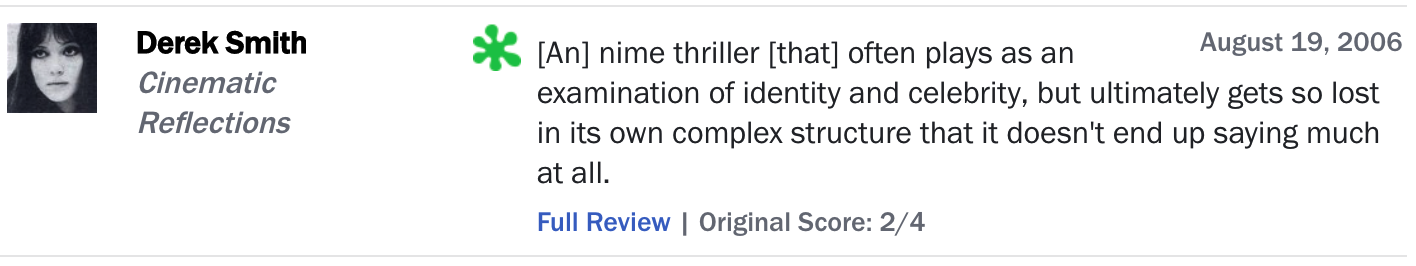
\includegraphics[width=0.5\linewidth]{image2.png}
\end{center}

Rotten Tomatoes ha clasificado estas reseñas como “positiva” y “negativa” respectivamente, como se indica por el tomate fresco e intacto en la reseña de arriba y la salpicadura de un tomate podrido en la reseña de abajo. En esta tarea, vas a crear un simple sistema de clasificación de texto que puede realizar esta tarea automáticamente. Vamos a considerar el siguiente conjunto de cuatro mini-reseñas, cada una etiquetada como positiva (+1) o negativa (-1):

\begin{enumerate}
    \item (-1) not good
    \item (-1) pretty bad
    \item (+1) good plot
    \item (+1) pretty scenery
\end{enumerate}

Cada reseña G es asignada a un vector de características \begin{math} \phi(x) \end{math}, el cuál asocia cada palabra a la cantidad de veces que aparece en la reseña. Por ejemplo, la segunda reseña se asigna al vector disperso de características \begin{math} \phi(x) = \end{math} \{pretty : 1, bad : 1\}. Recuerda la definición de la \textit{pérdida de articulación},

\begin{center}
    \begin{math}
        Loss_{hinge}(x,y,w) = 
    \end{math}
    max
    \begin{math}
        \{ 0,1-w * \phi(x)y \}
    \end{math}
    ,
\end{center}

donde \textit{x} es el texto de la reseña, \textit{y} es la clasificacion correcta y \textit{w} es el vector de pesos.

\begin{enumerate}
    \item Supongamos que corres el descenso de gradiente estocástico una vez por cada una de las cuatro reseñas de arriba en el mismo orden, actualizando los pesos de acuerdo a,
    
\begin{center}
    \begin{math}
        w \leftarrow w\nabla_w Loss_{hinge}(x,y,w).
    \end{math}
\end{center}
    
Después de las actualizaciones, ¿cuáles son los pesos de las seis palabras (“pretty”, “good”, “bad”, “plot”, “not”, “scenery”) que aparecen en las reseñas?
    
\end{enumerate}

\begin{itemize}
    \item utiliza \begin{math}
        \eta = 0.1
    \end{math}
    como tamaño de paso.

    \item inicializa \begin{math}
        w = [0,0,0,0,0,0]
    \end{math}
    .
    \item El gradiente \begin{math}
        \nabla_w Loss_{hinge}(x,y,w) = 0
    \end{math}
    cuando el margen es exactamente 1.
\end{itemize}



\begin{solution}
Como el \begin{math}
     \nabla_w Loss_{hinge}(x,y,w) = 0
\end{math}
es cero cuando el margen es exactamente 1, y dado que los valores iniciales de \textit{w} son ceros, la primera actualización de pesos no cambiará los valores de \textit{w} ya que el margen para todas las reseñas es 1 al principio.

\begin{enumerate}
    \item (-1) not good:
    
        \begin{math}
            Loss_{hinge}=(0,1-w*\eta(x)y) = max(0,1-[0,0,0,0,0,0]*{not : 1, bad : 1}*-1)=0
         \end{math}
    
    Como la perdida total es cero, no hay actualizacion.

    \item (-1) pretty bad:
        
        \begin{math}
            Loss_{hinge}=(0,1-w*\eta(x)y) = max(0,1-[0,0,0,0,0,0]*{pretty : 1, bad : 1}*-1)=2
         \end{math}

    \item (+1) good plot:

        \begin{math}
            Loss_{hinge}=(0,1-w*\eta(x)y) = max(0,1-[0,0,0,0,0,0]*{good : 1, plot : 1}*11)=0
         \end{math}

    \item (+1) good plot:

        \begin{math}
            Loss_{hinge}=(0,1-w*\eta(x)y) = max(0,1-[0,0,0,0,0,0]*{pretty : 1, scenery : 1}*11)=0
         \end{math}

    Tras estas actualizaciones, los pesos finales serian:

    \begin{math}
        w=[0.1,0.1,0,0,0,0]
    \end{math}
\end{enumerate}

\end{solution}

%%%%%%%%%%%%%%%%%%%%%%%%%%%%%%%%%
%% Desarrollando la intuición %%
%%%%%%%%%%%%%%%%%%%%%%%%%%%%%%%%%

\section*{Desarrollando la intuición}

Supongamos que ahora nos interesa predecir una calificación numérica para reseñas de películas. Utilizaremos un predictor no-lineal que toma una reseña G y regresa \begin{math}
    \epsilon(w*\phi(x))
\end{math}, donde

\begin{center}
    \begin{math}
        \epsilon(z)=(1+e^{-z})^{-1}
    \end{math}
\end{center}

es la función logística que aplasta un número real al rango ¹0• 1º. Para este problema, supón que la calificación de película \textit{y} es una variable con valor real en el rango [0,1].

\begin{enumerate}
    \item Supongamos que queremos usar la \textit{pérdida cuadrática}. Escribe la expresión para Loss(\textit{x,y,w}) para un dato(\textit{x,y}).

    \begin{solution}
        
    \end{solution}
\end{enumerate}

\end{document}
